\clearpage
\section{BB84 with Discrete Variables}

\begin{refsection}

\begin{tcolorbox}	
\begin{tabular}{p{2.75cm} p{0.2cm} p{10.5cm}} 	
\textbf{Students Name}  &:& Mariana Ramos (7/11/2017 - 9/4/2018) \\
                        & & Kevin Filipe (7/11/2017 - 10/11/2017) \\
\textbf{Starting Date} &:& November 7, 2017\\
\textbf{Goal}          &:& BB84 implementation with discrete variables.
\end{tabular}
\end{tcolorbox}

BB84 is a key distribution protocol which involves three parties, Alice, Bob and Eve. Alice and Bob exchange information between each other by using a quantum channel and a classical channel. The main goal is continuously build keys only known by Alice and Bob, and guarantee that eavesdropper, Eve, does not gain any information about the keys.


\subsection{Protocol Analysis}
\begin{tcolorbox}	
	\begin{tabular}{p{2.75cm} p{0.2cm} p{10.5cm}} 	
		\textbf{Students Name}  &:& Kevin Filipe (7/11/2017 - 10/11/2017)\\
		\textbf{Goal}          &:& BB84 - Protocol Description
	\end{tabular}
\end{tcolorbox}

BB84 protocol was created by Charles Bennett and Gilles Brassard in 1984 \cite{Bennet84}. It involves two parties, Alice and Bob, sharing keys through a quantum channel in which could be accessed by a eavesdropper, Eve. A basic model is depicted in figure \ref{fig:qkd model}.

\begin{figure}[H]
	\centering
	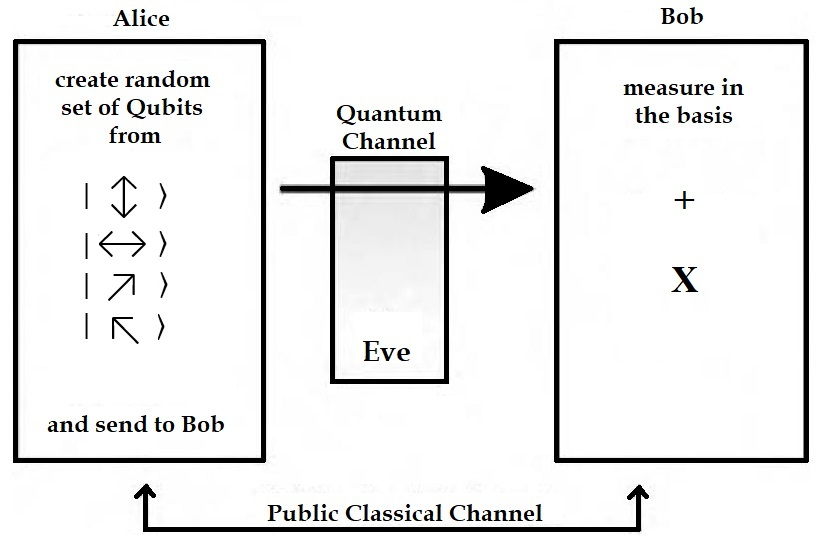
\includegraphics[width=0.8\textwidth,height=7cm]{./sdf/bb84_with_discrete_variables/figures/QKD_Model.png}
	\caption{Basic QKD Model. Alice and Bob are connected by 2 communication channels, a public quantum channel and a authenticated classical channel, with an eavesdropper, Eve (figure adapted from \cite{Gerry05}).}\label{fig:qkd model}
\end{figure}

We are going to analyse the BB84 protocol with bit encoding into photon state polarization. Two non-orthogonal basis are used to encode the information, the rectilinear and diagonal basis, + and x respectively. The following table shows this bit encoding.
\begin{table}[H]
	\centering
	\begin{tabular}{c|c|c}
		 Bit &  \textit{Rectilinear Basis,+} & \textit{Diagonal Basis,$\times$}\\ \hline
		0 &  0$º$ & -45$º$ \\
		1 & 90$º$ & 45$º$\\
	\end{tabular}
\end{table}

The protocol requires the following parameter and it is implemented with the following steps:

\begin{table}[hbt]
	\centering
	\caption{Initial Parameters.}
	\label{tb:param}
	\begin{tabular}{|c|c|}
		\hline
		\textbf{Parameter}  & \textbf{Description} 	   \\ \hline
			$M \times N$    & Scrambling Matrix M by N \\ \hline
			k				& Number of revealed bits for BER calculation \\ \hline
			$\alpha$        & Confidence level 	       \\ \hline
			    A    & B                \\ \hline
	\end{tabular}
\end{table}

\begin{enumerate}
	\item Alice generates two random bit strings. The random string , $R_{A1}$, corresponds to the data to be encoded into photon state polarization. $R_{A2}$ is a random string in which 0 and 1 corresponds to the rectilinear, +, and diagonal, $\times$, respectively.
	
	$$ R_{A1} = \{0,1,1,0,1,0,0,1,1,0,1,1,1,0,0,1,0,0,0,1\}$$
	\begin{eqnarray}
		R_{A2} &=& \{0,0,1,0,1,1,1,0,1,1,1,0,1,0,0,0,1,0,1,0\} \nonumber \\
		&=& \{+,+,\times,+,\times, \times, \times, +,\times, \times, \times,+,\times,+,+,+,\times,+,\times,+\}\nonumber
	\end{eqnarray}
	
	\item Alice transmits a train of photons, $S_{AB}$, obtained by encoding the bits, $R_{A1}$ with the respective photon polarization state $R_{A2}$.
	
	$$S_{AB} = \{\to, \uparrow, \searrow, \to, \searrow, \nearrow, \nearrow, \uparrow, \searrow, \nearrow, \searrow, \uparrow, \searrow, \to, \to, \uparrow, \nearrow, \to, \nearrow, \uparrow\}.$$
	
	\item Bob generates a random string, $R_{B}$, to receive the photon trains with the correspondent basis.
	\begin{eqnarray}
		R_{B} &=& \{0,1,1,1,0,1,0,0,1,1,0,0,1,1,0,0,1,1,0,0\} \nonumber\\
		&=&\{+,\times,\times,\times,+,\times,+,+,\times,\times,+,+,\times,\times,+,+,\times,\times,+,+\} \nonumber
	\end{eqnarray}
	
	\item Bob performs the incoming photon states measurement, $M_{B}$, with its generated random basis, $R_{B}$. If the two photon detectors don't click, means the bit was lost during transference due to attenuation. If both photon detectors click, a false positive was detected. In the measurements, $M_{B}$, the no-click in both detectors is represented by a -1 and the false positives to -2. The measurements done in rectilinear or diagonal basis are represented by 0 or 1, respectively. This is represented \ref{fig:bb84 detector}
	
	$$M_{B} = \{0,1,1,1,-1,1,0,0,-2,1,0,0,-2,1,0,0,1,-1,0,0\}$$	

	\begin{figure}[H]
		\centering
		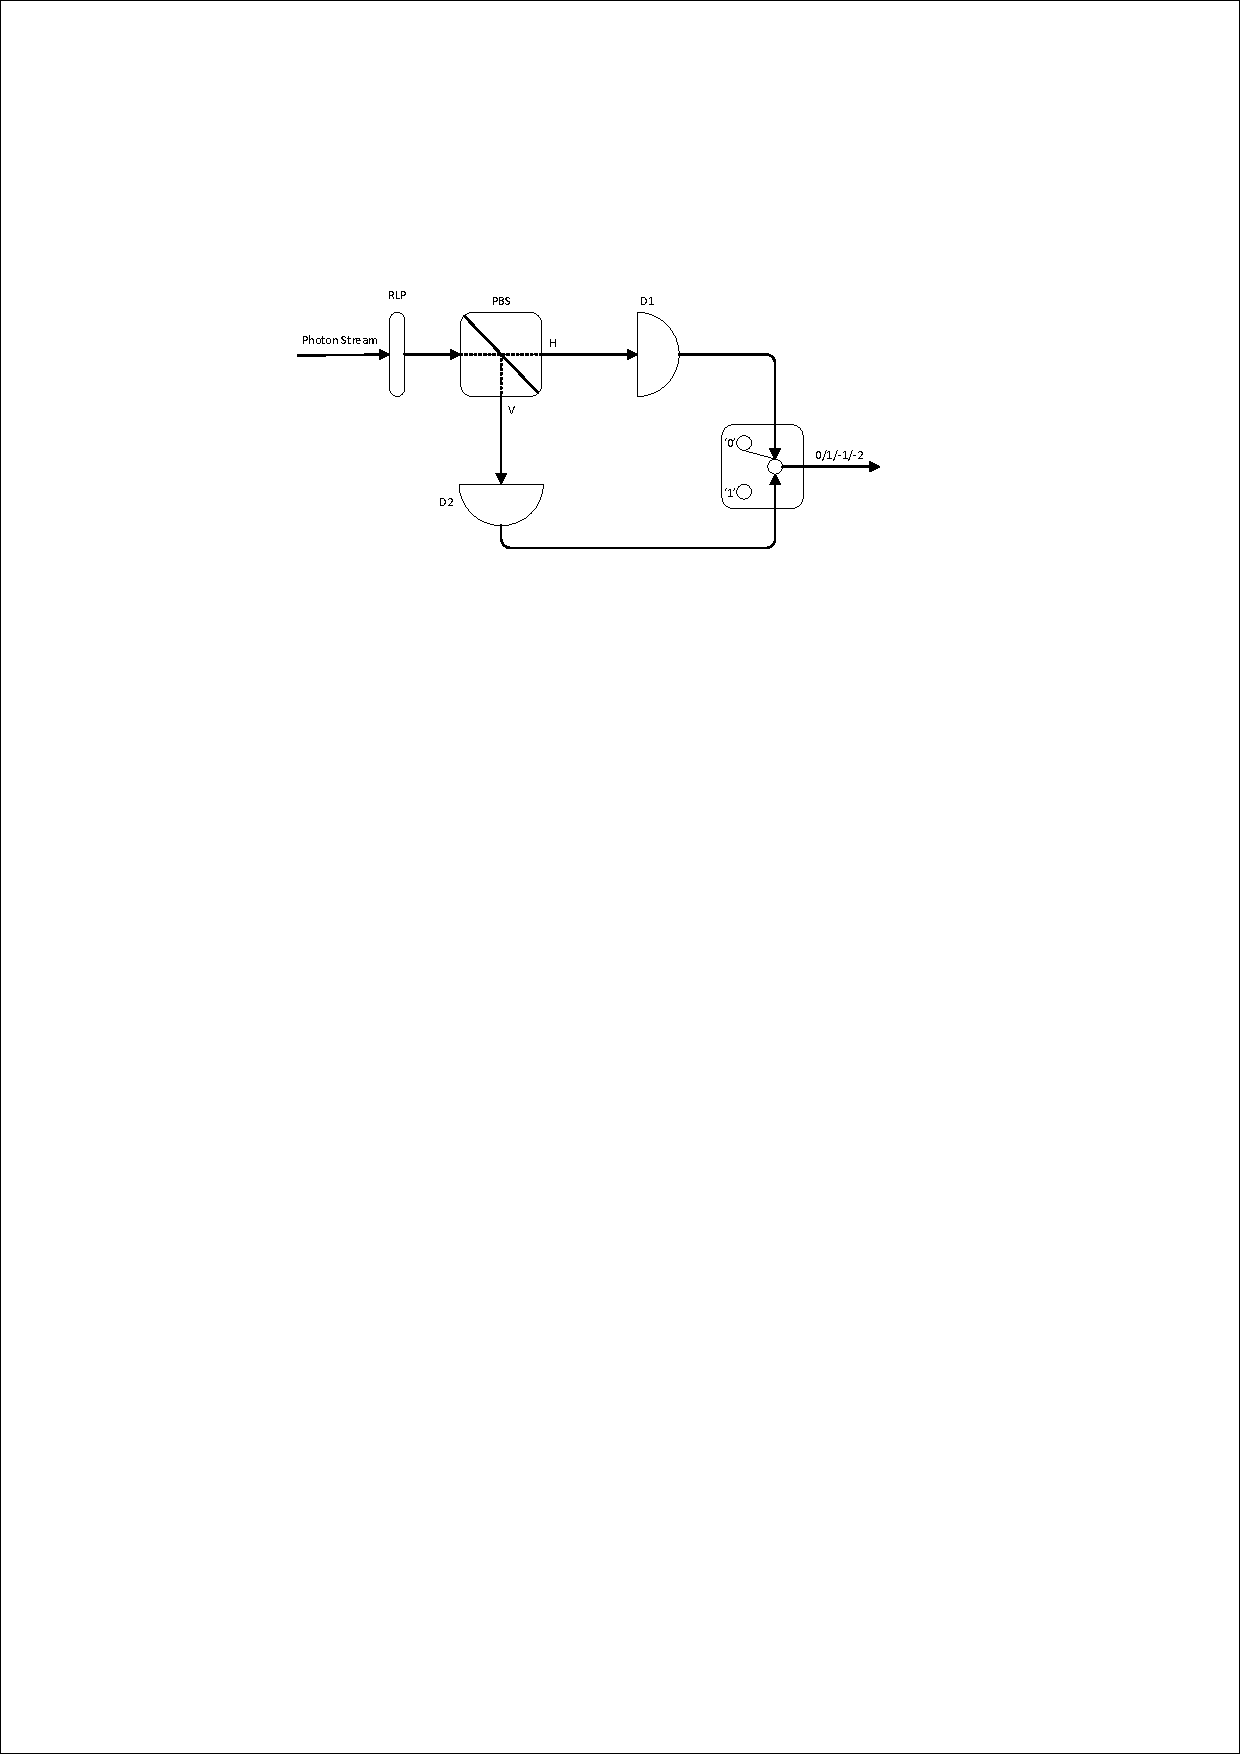
\includegraphics[width=0.8\textwidth,height=7cm]{./sdf/bb84_with_discrete_variables/figures/detector.png}
		\caption{Single-Photon Detection block with false-positives, -2, and attenuation, -1, detection depending on D1 and D2 output.\label{fig:bb84 detector}}
	\end{figure}
	
	\item After the measurement, Bob sends to Alice, using the classical channel, the used basis values, $R_{B}$ with the attenuation, -1, and false positives,-2.
	\item Alice performs a modified negated XOR, generating a sequence that detects when the same basis she used $B_{AB}$.
	
	\begin{table}[H]
		\centering
		\begin{tabular}{c|c c c c c c c c c c c c c c c c c c c c}
			$R_{A2}$ & 0 & 0 & 1 & 0 &  1 & 1 & 1 & 0 &  1 & 1 & 1 & 0 &  1 & 0 & 0 & 0 & 1 &  0 & 1 & 0 \\
			$R_{B}$  & 0 & 1 & 1 & 1 & -1 & 1 & 0 & 0 & -2 & 1 & 0 & 0 & -2 & 1 & 0 & 0 & 1 & -1 & 0 & 0 \\ \hline
			$B_{AB}$ & 1 & 0 & 1 & 0 &  0 & 1 & 0 & 1 &  0 & 1 & 0 & 1 &  0 & 0 & 1 & 1 & 1 &  0 & 0 & 1 \\
		\end{tabular}
	\end{table}

	\item Alice sends the $B_{AB}$ sequence to Bob, in which he can correlate with, $M_{B}$, and deduce the key $K_{AB}$.
	
			$$ K_{AB} = \{0,1,0,1,0,1,0,1,0,1\}.$$
	
	\item Alice then by having knowledge of $R_{A2}$ and $B_{AB}$ performs a scrambling algorithm over the deduced key. It is generated a matrix $M \times N$, according to the input parameter. Assuming a scrambling matrix of 3x4, \ref{tb:scram}. And being the scramble key represented as $KS_{AB}$
	
	\begin{table}[hbt]
		\centering
		\caption{Scrambling matrix}
		\label{tb:scram}
		\begin{tabular}{|c|c|c|c|c|}
			\hline
				0 & 1 & 0 & 1 \\ \hline
			    0 & 1 & 0 & 1 \\ \hline
				0 & 1 & - & - \\ \hline
		\end{tabular}
	\end{table}

	$$KS_{B} = \{0,0,0,1,1,1,0,0,1,1\}$$	
	
	\item Bob uses the same algorithm as Alice and scrambles his key.
	
	\item Bob then reveals a fixed number of his key to Alice. This number is also an input parameter value, k. With this the Quantum Bit Error Rate (QBER).
		
\end{enumerate}

	To determine the QBER, it is necessary to know the confidence interval parameter, $\alpha$ and the QBER limit, in which states the maximum allowed QBER by the user.
	Then to verify if the channel is reliable or not, the flowchart presented in figure \ref{fig:flowQber}.
	
	\begin{enumerate}
		\item Bob will reveals k bits sequence from the scrambled key, $SK_{AB}$ to Alice.
		\item Alice then returns to Bob the estimated QBER value, mQBER, with a confidence interval, [qLB, qUB] using the using the equations in the Bit Error Rate section, but applied to this protocol
		\item To check if the channel is compromised or not it is necessary to check if the QBER limit is higher than the QBER upper bound. If QBER limit is between the QBER lower and upper bound it is necessary to reveal more k bits from the key. Otherwise the channel is compromised and the key determination process needs to restart.
	\end{enumerate}
	
	
\begin{figure}[H]
	\centering
	\includegraphics[width=1\textwidth,height=7cm]{./sdf/bb84_with_discrete_variables/figures/qberEstimation.png}
	\caption{Flowchart to determine if the channel is reliable or not.}\label{fig:flowQber}
\end{figure}



\newpage

\subsection{Simulation Analysis}

\begin{tcolorbox}	
\begin{tabular}{p{2.75cm} p{0.2cm} p{10.5cm}} 	
\textbf{Students Name}  &:& Mariana Ramos (7/11/2017 - 9/4/2018) \\
\textbf{Goal}          &:& Perform a simulation of BB84 communication protocol.
\end{tabular}
\end{tcolorbox}

In this sub section the simulation setup implementation will be described in order to implement the BB84 protocol. In figure \ref{simulationimplemented} a top level diagram is presented. Then it will be presented the block diagram of the transmitter block (Alice) in figure \ref{alicesimulation} and the receiver block (Bob) in figure \ref{bobsimulation}. In a first approach, we do not consider the existence of eavesdropper.

\begin{figure}[H]
    \centering
        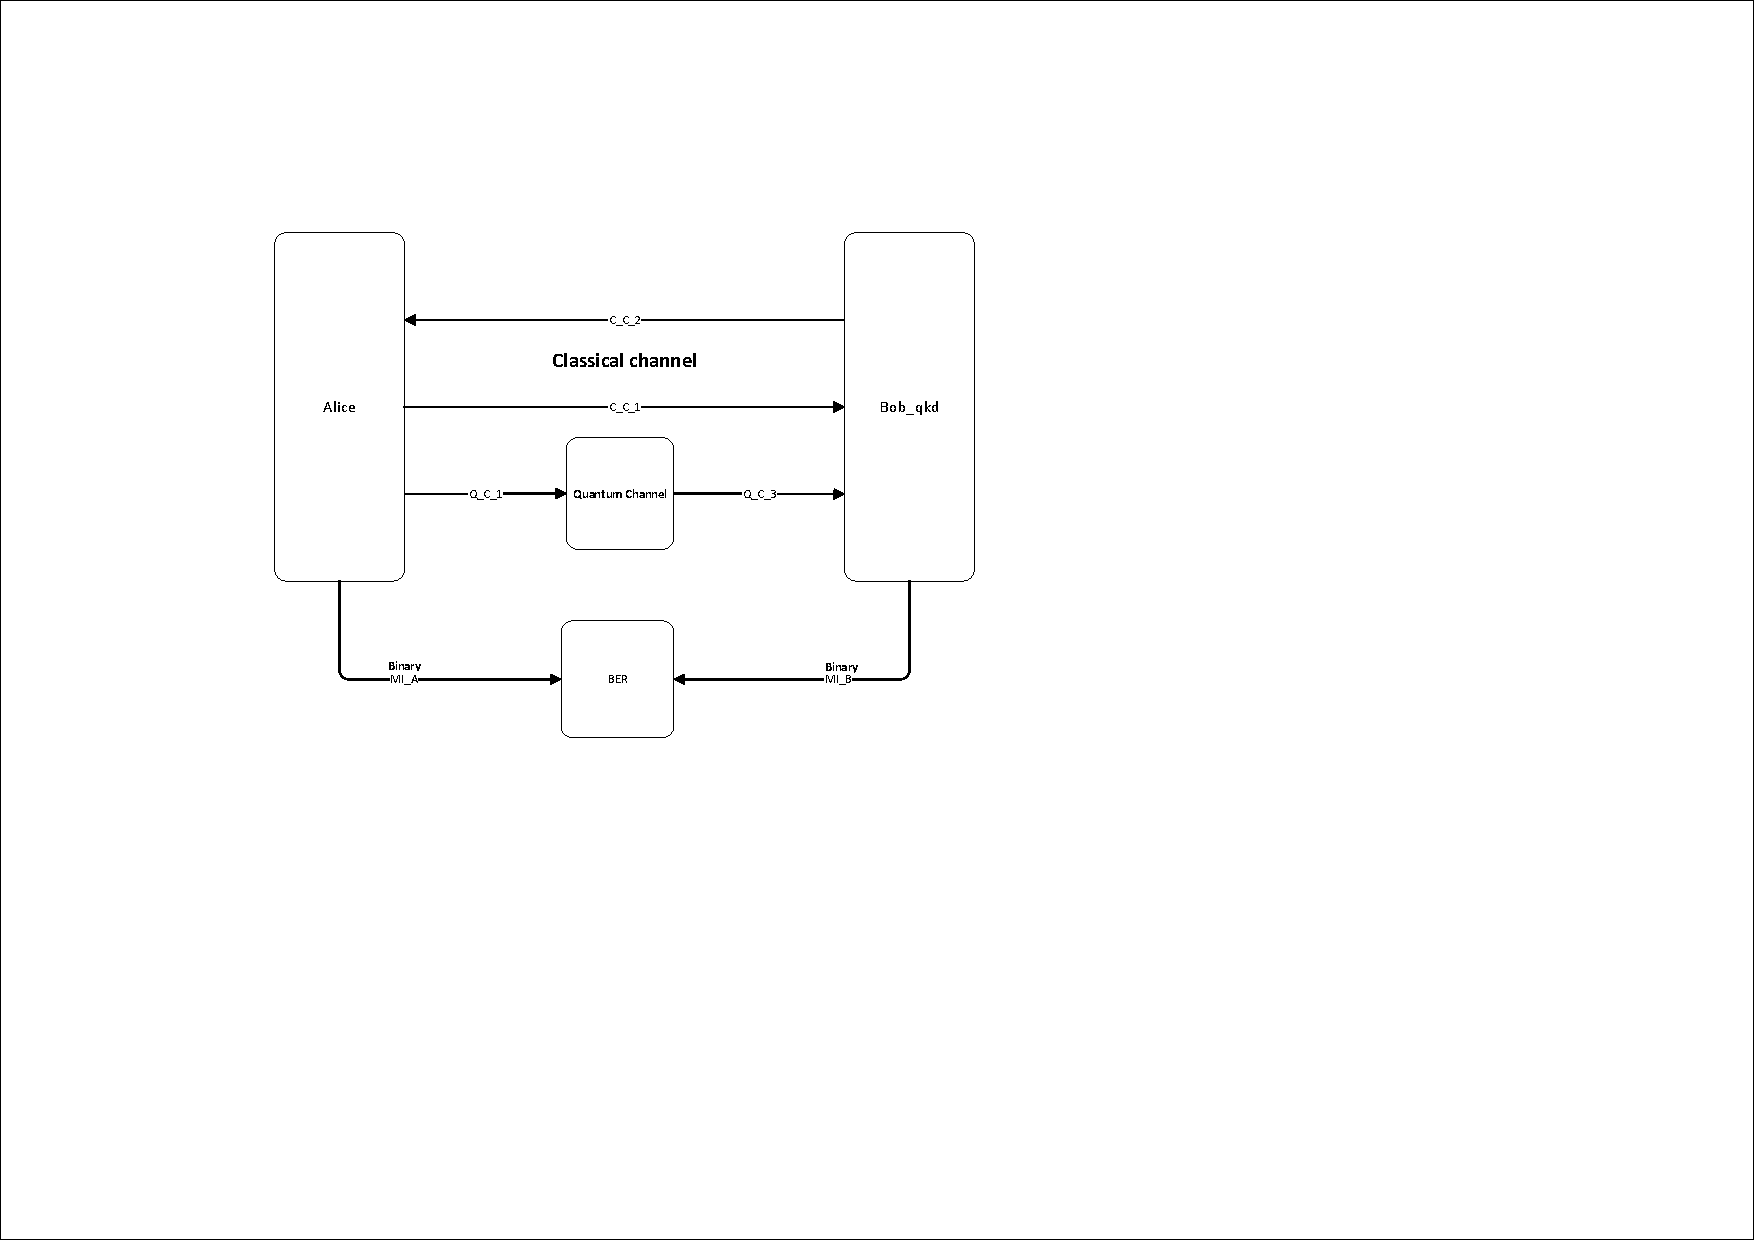
\includegraphics[clip, trim=1cm 8cm 10cm 3cm, width=1.00\textwidth]{./sdf/bb84_with_discrete_variables/figures/Simulation_toplevel_implemented.pdf}
    \caption{Simulation diagram at Alice's side}\label{simulationimplemented}
\end{figure}


Figure \ref{simulationimplemented} presents the top level diagram of our simulation. The setup contains two parties Alice and Bob, where the communication between them is done throughout two authenticated classical channels and one public quantum channel. In a first approach we will perform the simulation without eavesdropper presence. Furthermore, for bit error rate calculation between Alice and Bob.

\begin{figure}[h]
    \centering
        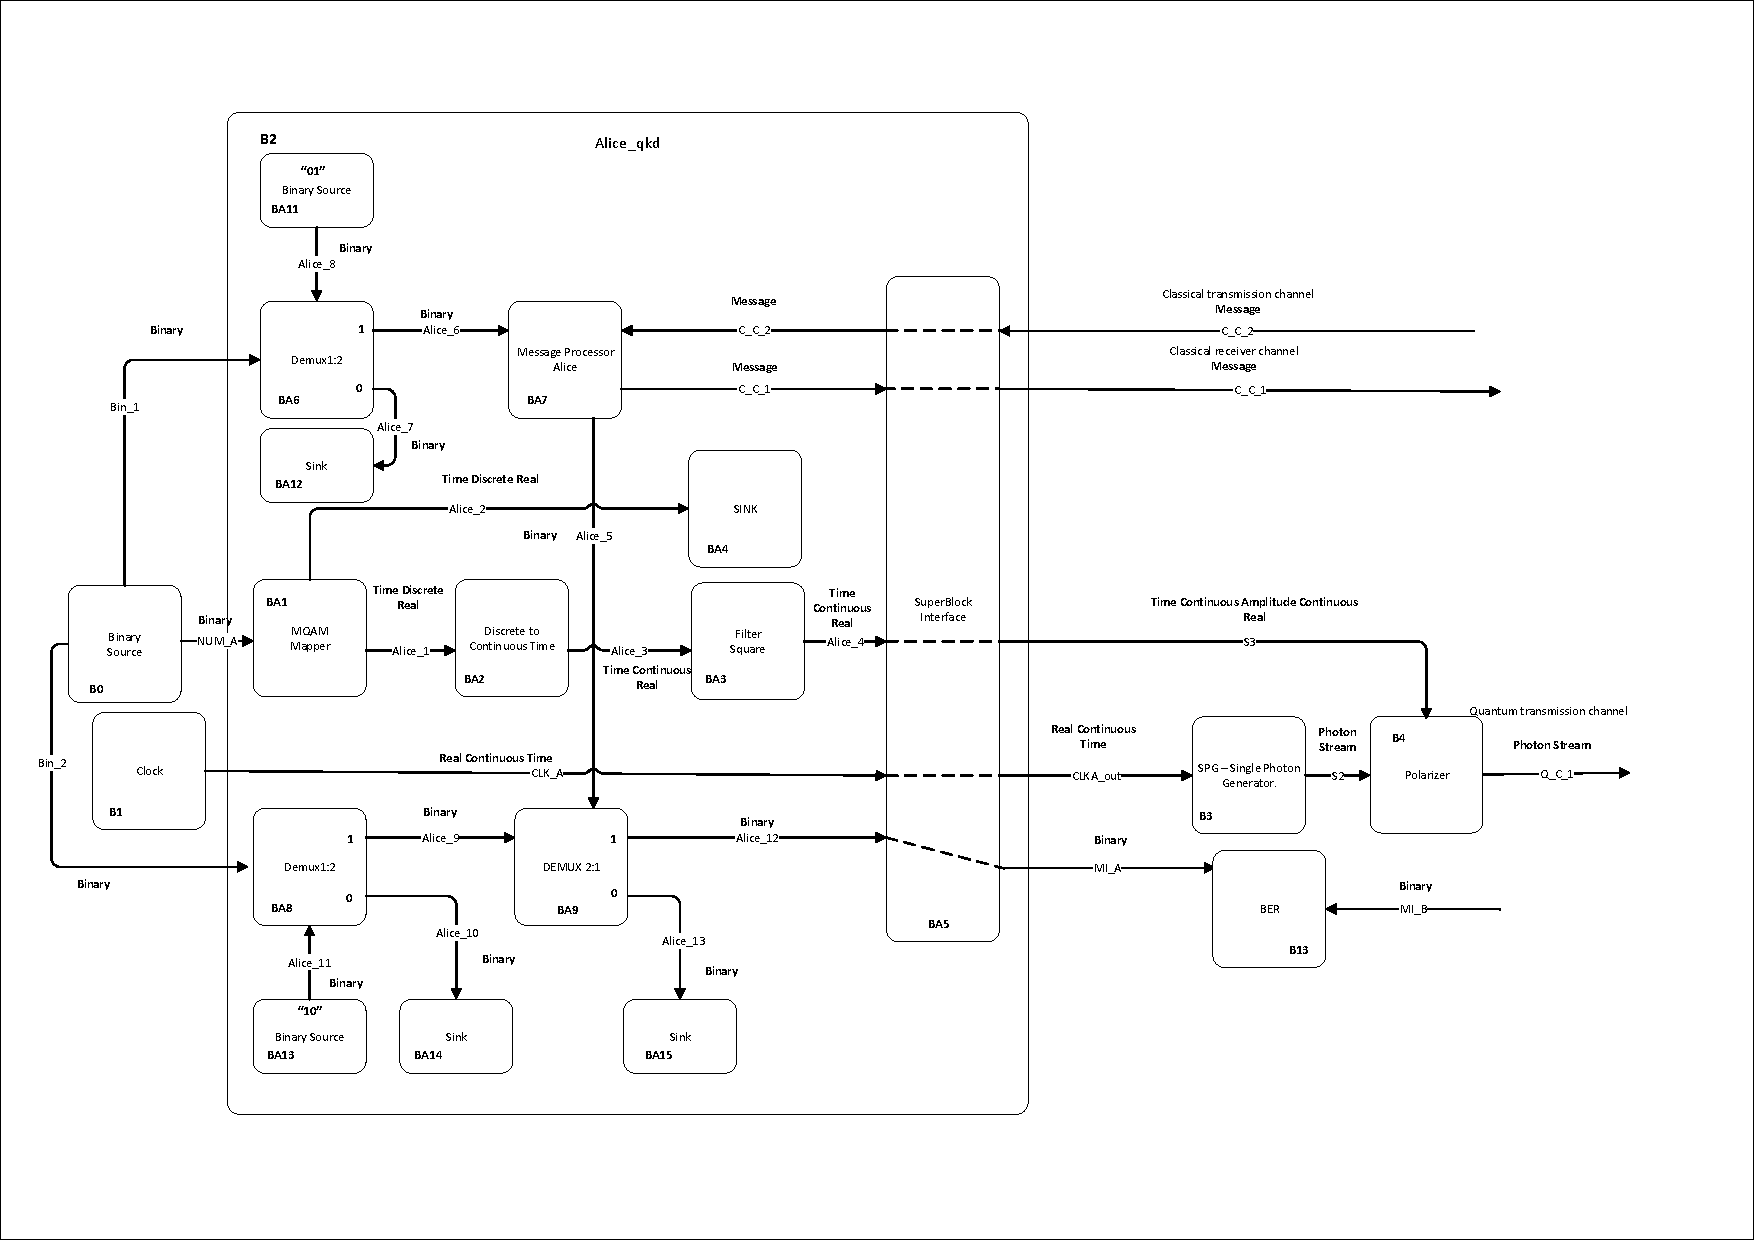
\includegraphics[clip, trim=0.5cm 1cm 0.5cm 1cm, width=1.10\textwidth]{./sdf/bb84_with_discrete_variables/figures/Simulation_Alice_bb84.pdf}
    \caption{Simulation diagram at Alice's side}\label{alicesimulation}
\end{figure}


\begin{figure}[h]
    \centering
        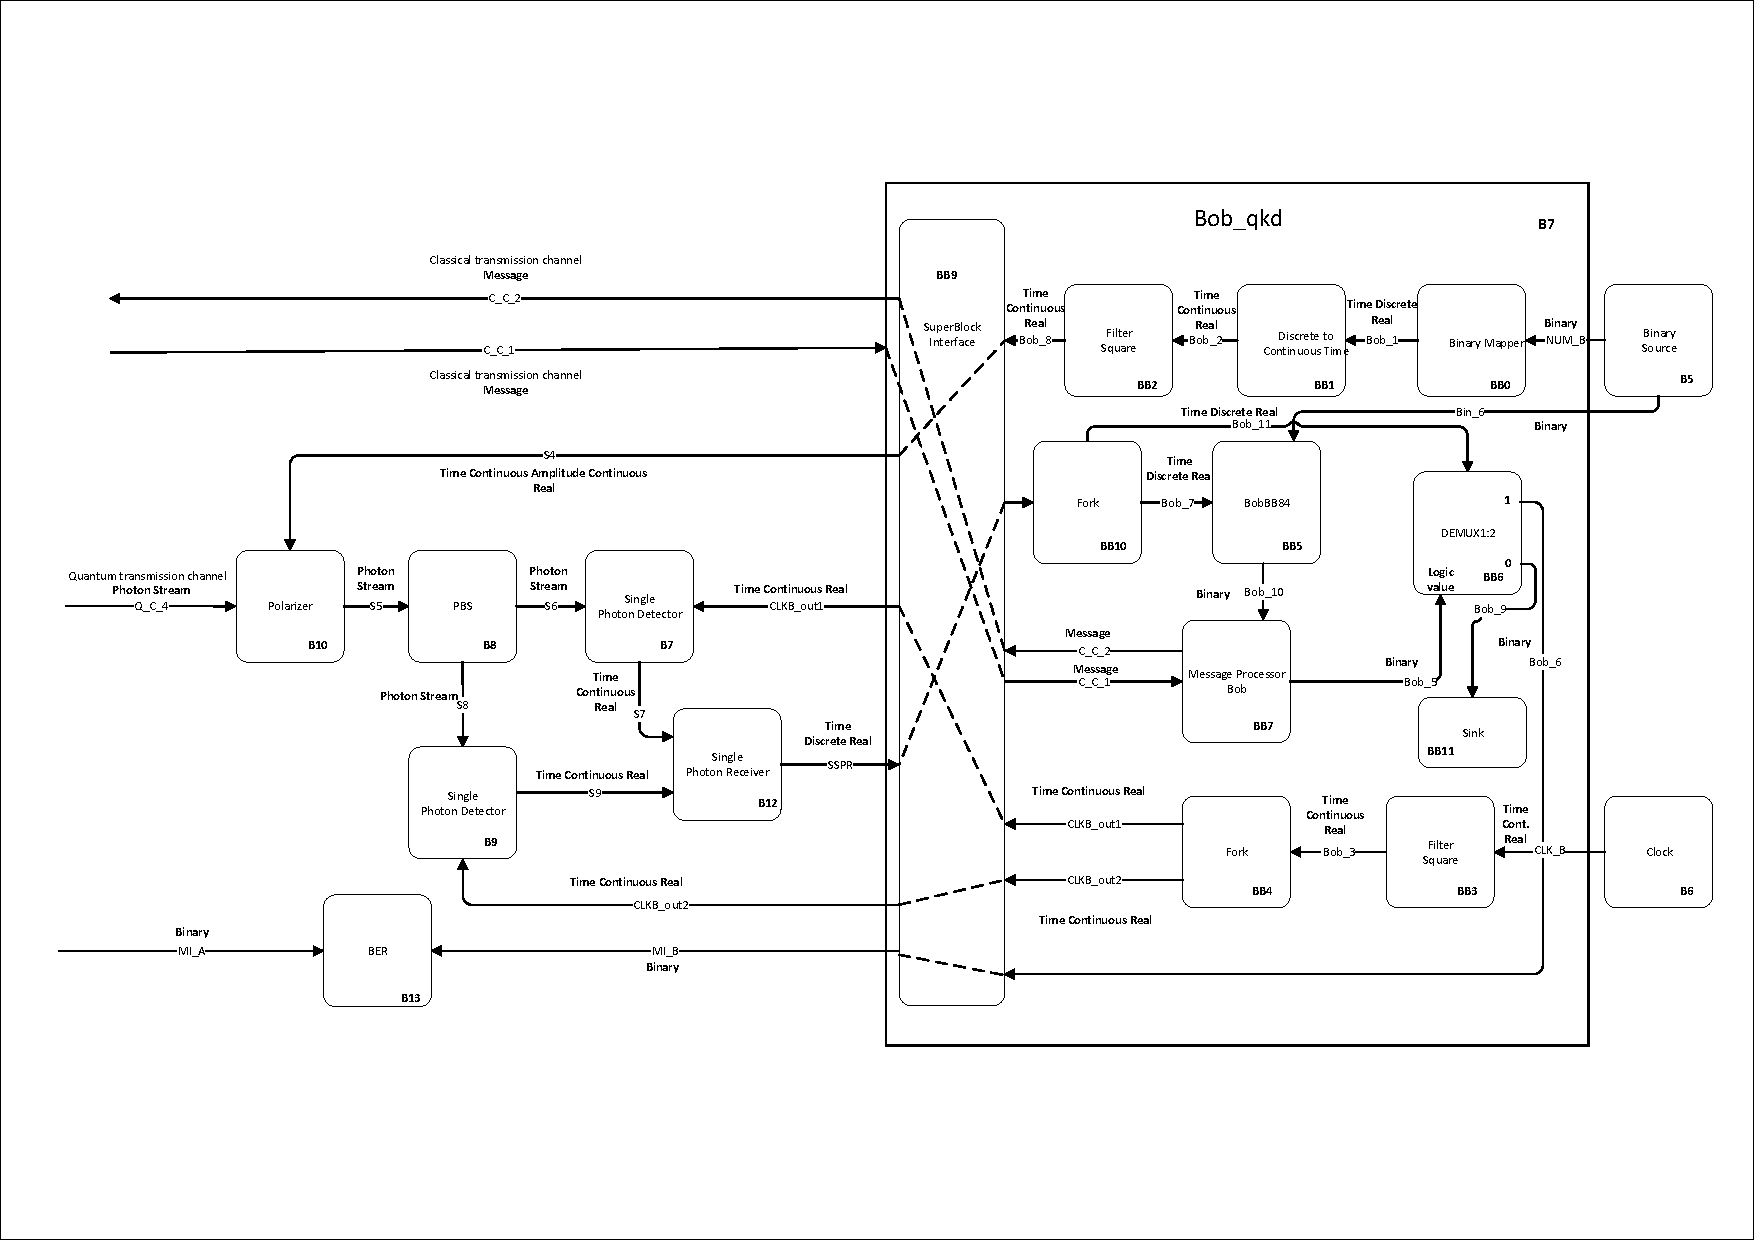
\includegraphics[clip, trim=0.5cm 2.0cm 0.5cm 0.5cm, width=1.00\textwidth]{./sdf/bb84_with_discrete_variables/figures/Simulation_Bob_bb84.pdf}
    \caption{Simulation diagram at Bob's side}\label{bobsimulation}
\end{figure}

    In figure \ref{alicesimulation} one can observe a block diagram of the simulation at Alice's side. As it is shown in the figure, Alice must have one block for random number generation which is responsible for basis generation to polarize the photons, and for key random generation in order to have a random state to encode each photon. Furthermore, she has a Processor block for all logical operations: array analysis, random number generation requests, and others. This block also receives the information from Bob after it has passed through a fork's block. In addition, it is responsible for set the initial length $l$ of the first array of photons which will send to Bob. This block also must be responsible for send classical information to Bob. Finally, Processor block will also send a real continuous time signal to single photon generator, in order to generate photons according to this signal, and finally this block also sends to the polarizer a real discrete signal in order to inform the polarizer which basis it should use. Therefore, she has two more blocks for quantum tasks: the single photon generator and the polarizer block which is responsible to encode the photons generated from the previous block and send them throughout a quantum channel from Alice to Bob.

    Finally, Alice's processor has an output to Mutual Information top level block, $Ms_{A}$.

    In figure \ref{alicesimulation} one can observe a block diagram of the transmitter. As it is shown in the figure, the transmitter must have one block for random number generation (binary source) which is responsible for basis generation to polarize the photons, and for key random generation in order to have a random state to encode each photon. This block has three outputs which will be inputs for the super block Alice. Furthermore, Alice block is responsible for all logical operations: random single photons state values generation, receive and send messages to the receiver Bob by using the classical channels, binary output for mutual information calculations. Each block of the super block is described in Library chapter. Finally, Alice block will also send a real continuous time signal to single photon generator (clock sets the rate oh photons generation), in order to generate photons polarized in the horizontal axis by default. Therefore, the transmitter has one more block, the polarizer block, which is responsible to encode the photons generated from the previous block and send them throughout a quantum channel from Alice to Bob.

     In figure \ref{bobsimulation} one can see a block diagram of the simulation for receiver (Bob). The receiver has one block for Random Number Generation which is responsible for randomly generate basis values which Bob will use to measure the photons sent by Alice throughout the quantum channel. Like transmitter, the receiver has the Bob block responsible for receive and send messages through the classical channel, receive single photons values detection from the single photon detectors, provides a clock signal to the detectors and send binary values for mutual information calculation. Furthermore, the receiver has two blocks for single photon detection (one for horizontal detection and other for vertical detection) which receives from Bob block a real continuous time signal which will set the detection window for the detector and outputs for Bob block the result value for detection. In addition, there is a polarizer which receives from Bob block a time continuous real signal which provides information about the rotation angle. If the basis chosen by Bob is the diagonal basis he sends "$45^\circ$", otherwise sends "$0^\circ$". The polarization beam splitter divides the input photon stream in horizontal component and vertical component.




%\begin{figure}[h]
%	\centering
%	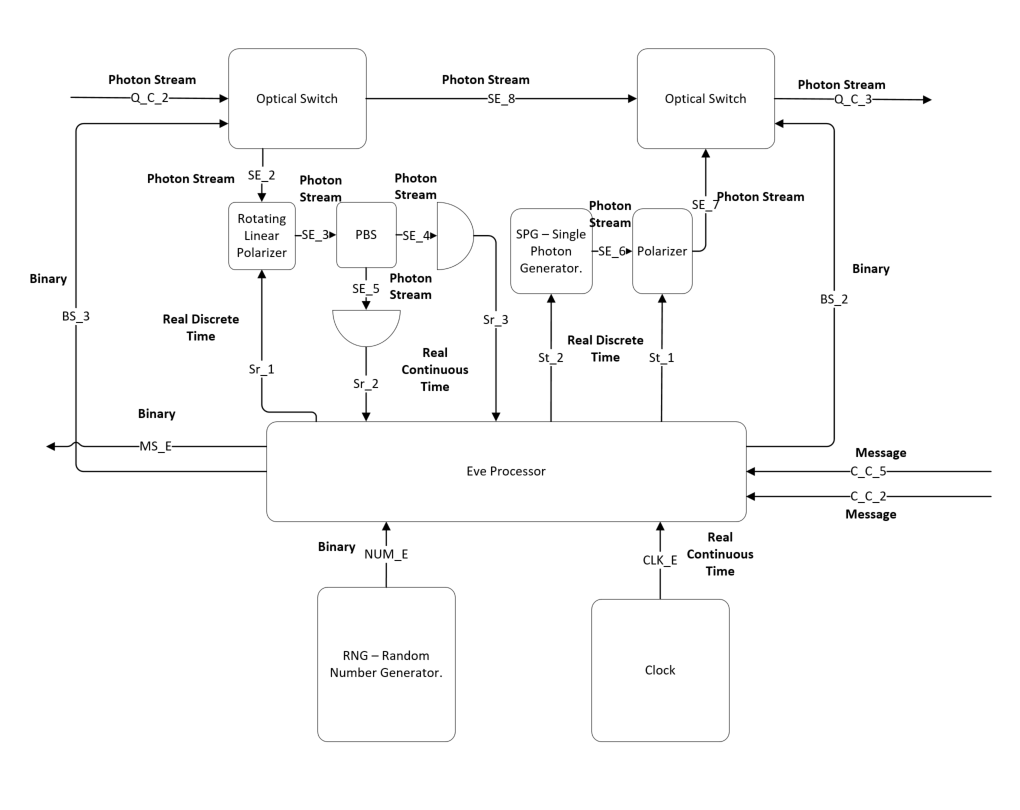
\includegraphics[width=1.1\textwidth, height=14cm]{./sdf/bb84_with_discrete_variables/figures/eve_simulation.png}
%	\caption{Simulation diagram at Eve's side}\label{evesimulation}
%\end{figure}
%
%Figure \ref{evesimulation} presents the Eve's side diagram. Eve's processor has two receiver classical signals, one from Alice (\textbf{C\_C\_2}) and other from Bob (\textbf{C\_C\_5}). About quantum channel, Eve received a quantum message from Alice through the channel \textbf{Q\_C\_1} and depends on her decision the photon can follows directly to Bob or the photon's state can be changed by her. In this case, the photon is received by a block similar to Bob's diagram \ref{bobsimulation} and this block sends a message to Eve's processor in order to reveal the measurement result. After that, Eve's processor sends a message to Alice's diagram similar to figure \ref{alicesimulation} and this block is responsible for encode the photon in a new state. Now, the changed photon is sent to Bob.
%
%In addition, Eve's diagram has one more output $Ms_{E}$ which is a message sent to the mutual information block as an input parameter.

\begin{table}[H]
\centering
\caption{System Signals}
\label{tb:signals}
\begin{tabular}{|c|c|c|}
\hline
\textbf{Signal name}                        & \textbf{Signal type}                      \\ \hline
NUM\_A, NUM\_B, Bin\_1, Bin\_2, Bin\_6      &  Binary                                   \\ \hline
MI\_A, MI\_B                                &  Binary                                   \\ \hline
CLK\_A, CLK\_B                              &  TimeContinuousAmplitudeContinuous        \\ \hline
CLK\_A\_out, CLKB\_out1, CLKB\_out2         &  TimeContinuousAmplitudeContinuous        \\ \hline
S2, S5, S6, S8                              &  PhotonStreamXY                           \\ \hline
S3, S7, S9                                  &  TimeContinuousAmplitudeDiscreteReal      \\ \hline
S4                                          &  TimeContinuousAmplitudeContinuousReal      \\ \hline
C\_C\_1, C\_C\_3                            &  Messages                                 \\ \hline
C\_C\_6, C\_C\_4                            &  Messages                                 \\ \hline
Q\_C\_1, Q\_C\_4                            &  PhotonStreamXY                           \\ \hline

\end{tabular}
\end{table}

Table \ref{tb:signals} presents the system signals as well as them type.

\begin{table}[H]
\centering
\caption{System Input Parameters}
\label{tb:inputparameters}
\begin{tabular}{|c|c|c|}
\hline
\textbf{Parameter}                      & \textbf{Default Value}                                & \textbf{Description} \\ \hline
rateOfPhotons                           & 1000 photons/s                                        &  Number of photon per sample.\\ \hline
iqAmplitudeValues                       & \{-45,0\},\{0,0\},\{45,0\},\{90,0\}                   &  Possible photon states. \\ \hline
numberOfSamplesPerSymbol                & 16                                                    &  Number of samples per symbol. \\ \hline
detectorWindowTimeOpen                  & 0.2 ms                                                & smaller than 1 ms \\ \hline
detectorPulseDelay                      & 0.7 ms                                                & in units of ms \\ \hline
detectorProbabilityDarkCount            & 0.0                                                   &  Probability of dark counts  \\
                                        &                                                       &  in single-photon detector.  \\ \hline
rotationAngle                           & 0.0                                                   & Polarization angle in XY axis   \\
                                        &                                                       & to introduce in Deterministic \\
                                        &                                                       & SOP changes.\\ \hline
elevationAngle                          & 0.0                                                   & Polarization angle in Poincare \\
                                        &                                                       &  sphere to introduce in \\
                                        &                                                       &  Deterministic SOP changes.\\ \hline
fiberLength                             & 10 km                                                    &  Length of the optical fibre in km. \\ \hline
fiberAttenuation                        & 0.2 dB/km                                               &  Attenuation of the optical fibre \\
                                        &                                                       &  in dB/km.  \\ \hline

\end{tabular}
\end{table}

\begin{table}[H]
\centering
\caption{Header Files}
\label{tb:signals}
\begin{tabular}{|c|c|c|}
\hline
\textbf{File name}                                          & \textbf{Description} & \textbf{Status} \\ \hline
netxpto\_20180118.h                                         &                      &    \checkmark      \\ \hline
alice\_qkd\_20180409.h                                      &                      &    \checkmark      \\ \hline
binary\_source\_20180118.h                                  &                      &    \checkmark      \\ \hline
bob\_qkd\_20180409.h                                        &                      &    \checkmark      \\ \hline
clock\_20171219.h                                           &                      &    \checkmark      \\ \hline
discrete\_to\_continuous\_time\_20180118.h                  &                      &    \checkmark      \\ \hline
m\_qam\_mapper\_20180118.h                                  &                      &    \checkmark      \\ \hline
polarization\_beam\_splitter\_20180109.h                    &                      &    \checkmark      \\ \hline
polarization\_rotator\_20180113.h                           &                      &    \checkmark      \\ \hline
pulse\_shaper\_20180111.h                                   &                      &    \checkmark      \\ \hline
single\_photon\_detector\_20180206.h                        &                      &    \checkmark      \\ \hline
single\_photon\_receiver\_20180303.h                        &                      &    \checkmark      \\ \hline
SOP\_modulator\_20180319.h                                  &                      &    \checkmark      \\ \hline
coincidence\_detector\_20180206.h                           &                      &    \checkmark      \\ \hline
single\_photon\_source\_20171218.h                          &                      &    \checkmark      \\ \hline
sink\_20180118.h                                            &                      &    \checkmark      \\ \hline
super\_block\_interface\_20180118.h                         &                      &    \checkmark      \\ \hline
message\_processor\_alice\_20180205.h                       &                      &    \checkmark      \\ \hline
demux\_1\_2\_20180205.h                                     &                      &    \checkmark      \\ \hline
binary\_mapper\_20180205.h                                  &                      &    \checkmark      \\ \hline
bobBB84\_20180221.h                                         &                      &    \checkmark      \\ \hline
message\_processor\_bob\_20180221.h                         &                      &    \checkmark      \\ \hline
sampler\_20171119.h                                         &                      &    \checkmark      \\ \hline
optical\_attenuator\_20180304.h                             &                      &    \checkmark      \\ \hline
fork\_20180112.h                                            &                      &    \checkmark      \\ \hline
\end{tabular}
\end{table}

\begin{table}[H]
\centering
\caption{Source Files}
\label{tb:signals}
\begin{tabular}{|c|c|c|}
\hline
\textbf{File name}                                          & \textbf{Description} & \textbf{Status}    \\ \hline
netxpto\_20180118.cpp                                       &                      &    \checkmark      \\ \hline
bb84\_with\_discrete\_variables\_sdf.cpp                    &                      &    \checkmark      \\ \hline
alice\_qkd\_20180409.cpp                                    &                      &    \checkmark      \\ \hline
binary\_source\_20180118.cpp                                &                      &    \checkmark      \\ \hline
bob\_qkd\_20180409.cpp                                      &                      &    \checkmark      \\ \hline
clock\_20171219.cpp                                         &                      &    \checkmark      \\ \hline
discrete\_to\_continuous\_time\_20180118.cpp                &                      &    \checkmark      \\ \hline
m\_qam\_mapper\_20180118.cpp                                &                      &    \checkmark      \\ \hline
polarization\_beam\_splitter\_20180109.cpp                  &                      &    \checkmark      \\ \hline
polarization\_rotator\_20180113.cpp                         &                      &    \checkmark      \\ \hline
pulse\_shaper\_20180111.cpp                                 &                      &    \checkmark      \\ \hline
single\_photon\_detector\_20180206.cpp                      &                      &    \checkmark      \\ \hline
single\_photon\_receiver\_20180303.cpp                      &                      &    \checkmark      \\ \hline
SOP\_modulator\_20180319.cpp                                &                      &    \checkmark      \\ \hline
coincidence\_detector\_20180206.cpp                         &                      &    \checkmark      \\ \hline
single\_photon\_source\_20171218.cpp                        &                      &    \checkmark      \\ \hline
sink\_20180118.cpp                                          &                      &    \checkmark      \\ \hline
super\_block\_interface\_20180118.cpp                       &                      &    \checkmark      \\ \hline
message\_processor\_alice\_20180205.cpp                     &                      &    \checkmark      \\ \hline
demux\_1\_2\_20180205.cpp                                   &                      &    \checkmark      \\ \hline
binary\_mapper\_20180205.cpp                                &                      &    \checkmark      \\ \hline
bobBB84\_20180221.cpp                                       &                      &    \checkmark      \\ \hline
message\_processor\_bob\_20180221.cpp                       &                      &    \checkmark      \\ \hline
sampler\_20171119.cpp                                       &                      &    \checkmark      \\ \hline
optical\_attenuator\_20180304.cpp                           &                      &    \checkmark      \\ \hline
fork\_20180112.cpp                                          &                      &    \checkmark      \\ \hline
\end{tabular}
\end{table}

\subsubsection{Simulation Results}

Figure \ref{toplevelalicebob} represents the block diagram of the first simulation performed between Alice and Bob. This simulation intends to simulate the communication protocol between Alice and Bob until they do the Basis Reconciliation. At this time, it is not taken into account any attack from an eavesdropper. However, as one can learn from theoretical protocol analysis, the attenuation due the fiber losses, dark counts probabilities from single photon detectors and the SOP drift over the quantum channel are all taken into account.

\begin{figure}[h]
    \centering
        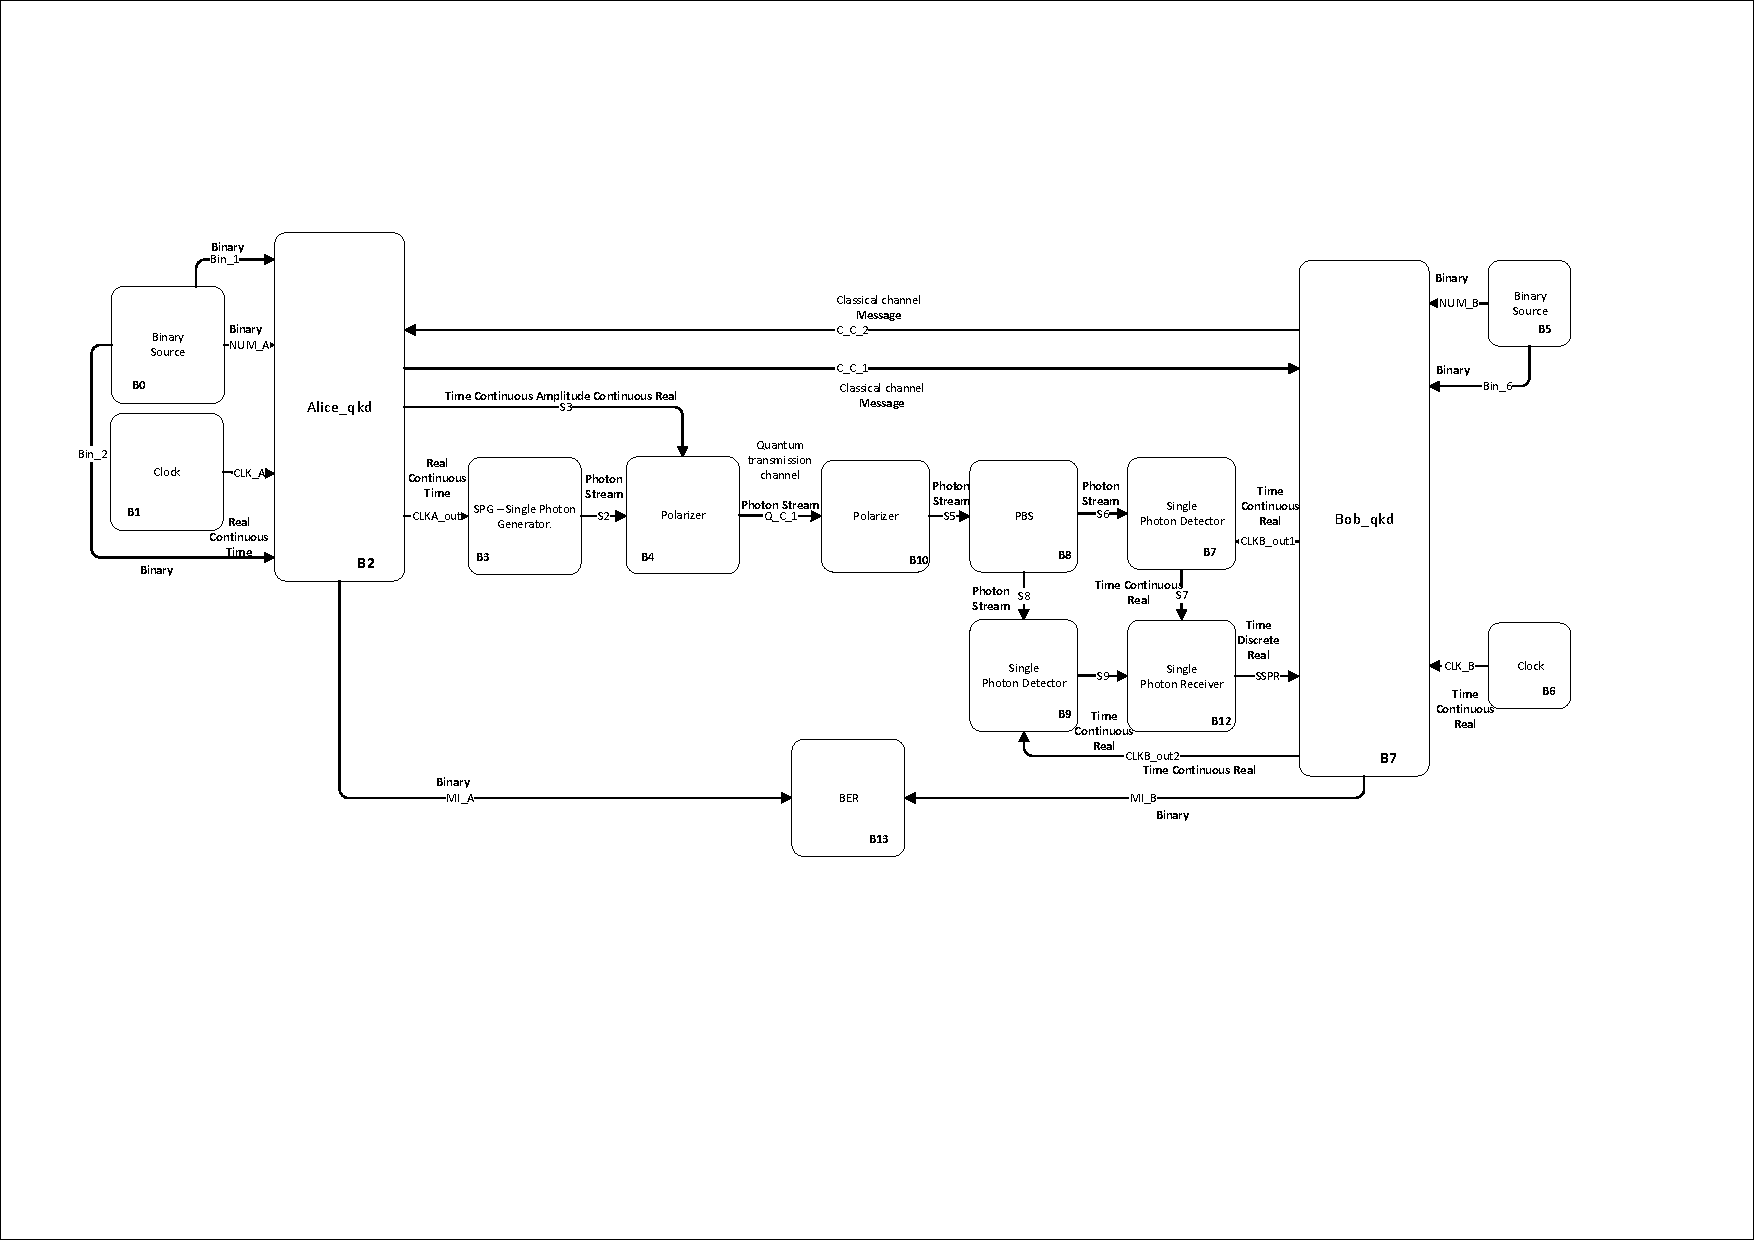
\includegraphics[clip=true, trim=1.2cm 5.0cm 0.5cm 2.5cm, width=1.10\textwidth]{./sdf/bb84_with_discrete_variables/figures/Simulation_toplevel_bb84.pdf}
    \caption{Diagram block of simulation performed between Alice and Bob until Basis Reconciliation. }\label{toplevelalicebob}
\end{figure}

Alice starts by sending a sequence of photons to Bob, and then he measures the photons according to random basis randomly generated by his binary source. After that, he follows the protocol described above until Alice sends to him a string of '0' and '1' where '0' means that both used different basis and '1' means that they used the same basis. Therefore, Alice and Bob outputs a binary signal "MI\_A" and "MI\_B", respectively. In case of no errors occurred in the quantum channel, these signals should be equal in order to both have the same sequence of bits. Furthermore, QBER between the two sequences should be $0$. This way, Alice can encode messages using these keys and Bob will be capable of decrypt the message using these symmetric keys. When errors are introduced in quantum channel QBER value will increase as we can see later.

\begin{figure}[H]
    \centering
        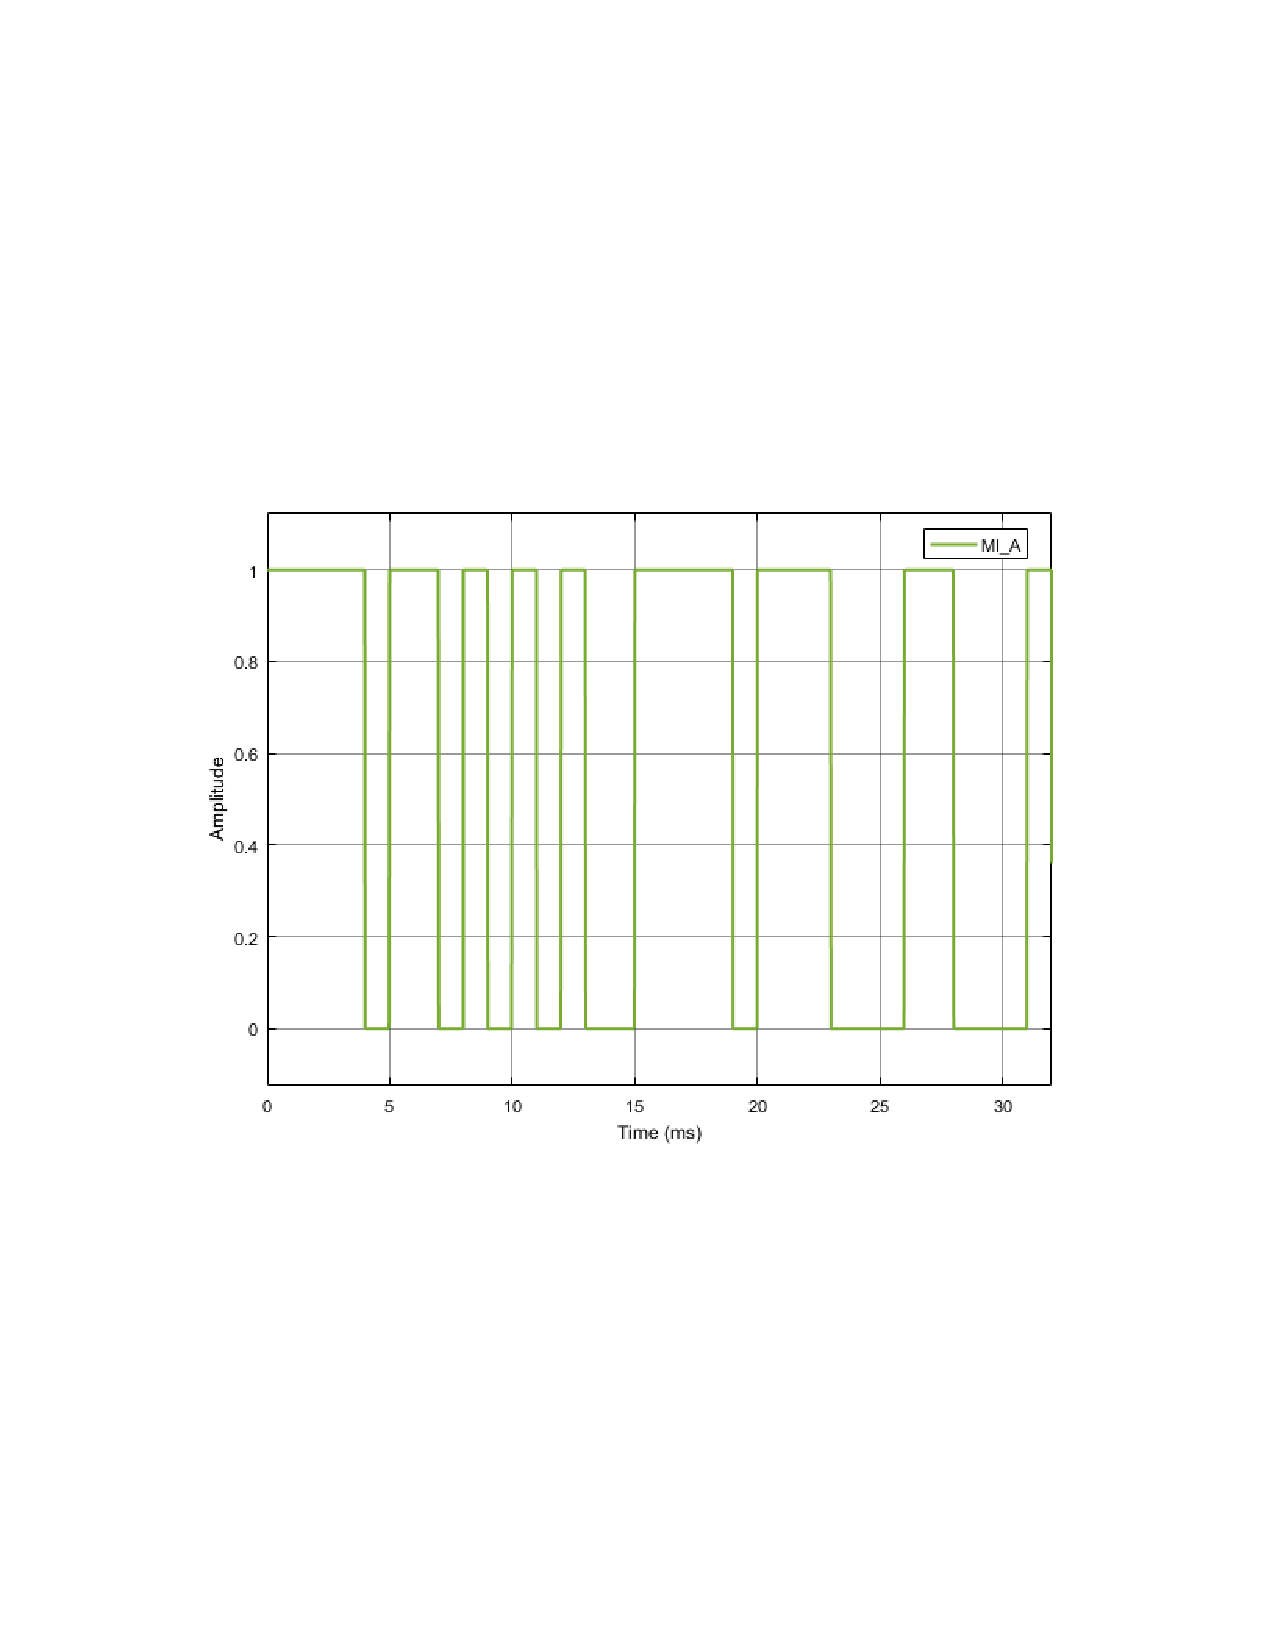
\includegraphics[clip, trim=3cm 9.0cm 2cm 7cm, width=0.50\textwidth]{./sdf/bb84_with_discrete_variables/figures/mia.pdf}
    \caption{MI\_A signal. }\label{mia}
\end{figure}

Figure \ref{mia} and figure \ref{mib} represent the sequence of bits which will be used by Alice to encode the messages and the sequence of bits used by Bob to decode the message when no errors in quantum channel are taken into account, respectively. As one can see the two signals are equal which meets the expected result. In this way, the first step of the protocol has been achieved.

\begin{figure}[h]
    \centering
        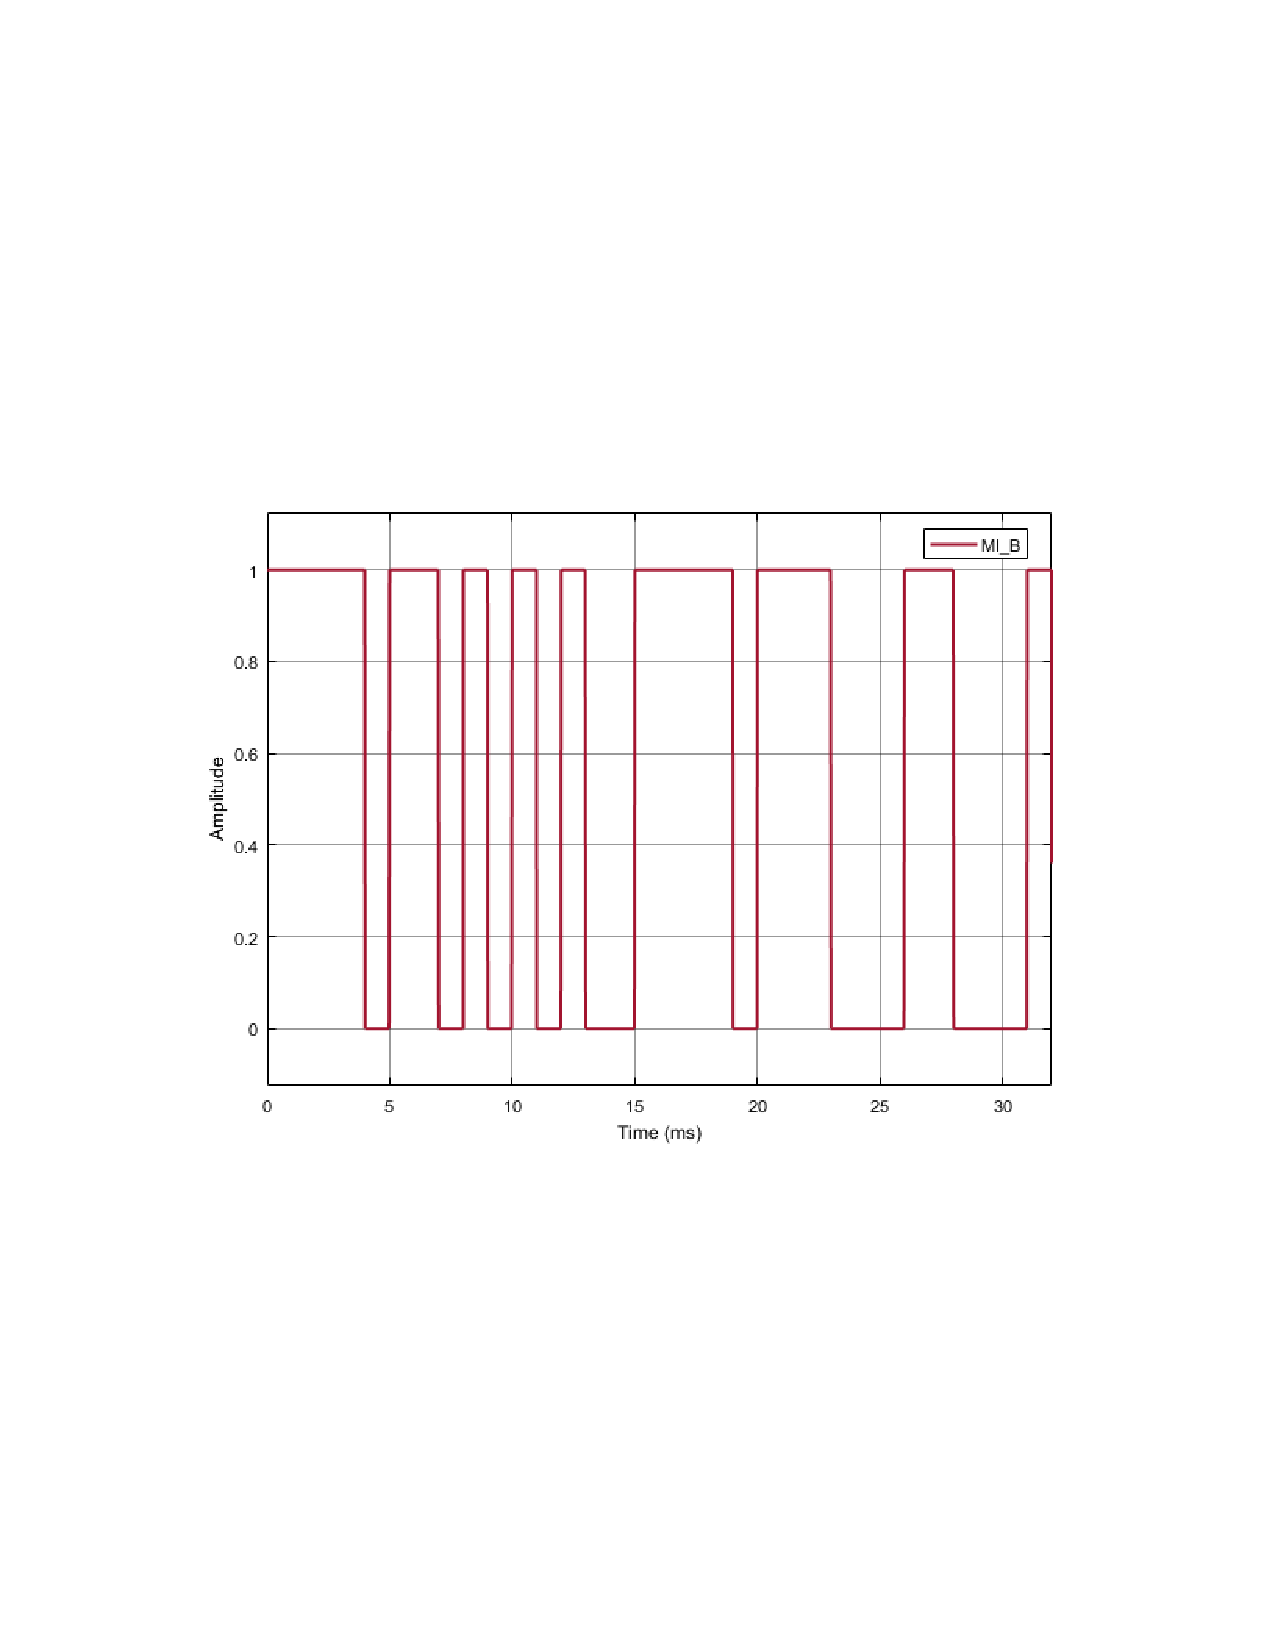
\includegraphics[clip, trim=3cm 9.5cm 2cm 7cm, width=0.50\textwidth]{./sdf/bb84_with_discrete_variables/figures/mib.pdf}
    \caption{MI\_B signal. }\label{mib}
\end{figure}

As one can see in figure \ref{toplevelsimulation} a block which calculates QBER is connected to Alice and Bob. This block calculates the QBER between the measurements that Bob performed with the same basis as Alice, based on method described in \cite{Muga11}. Thus, as expected, the QBER is $0 \%$ when no errors are taken into account.

Next, some errors due the changes in state of polarization of the single photons transmitted between Alice and Bob were added. This way, a polarization rotator in the middle of the quantum channel was added, which is controlled by a SOP modulator block as it is shown in figure \ref{sop_channel} with modelled with deterministic \cite{Muga15} and stochastic \cite{Czegledi16} methods. Additional information about the blocks presented in this quantum channel can be found in library chapter.

\begin{figure}[h]
    \centering
        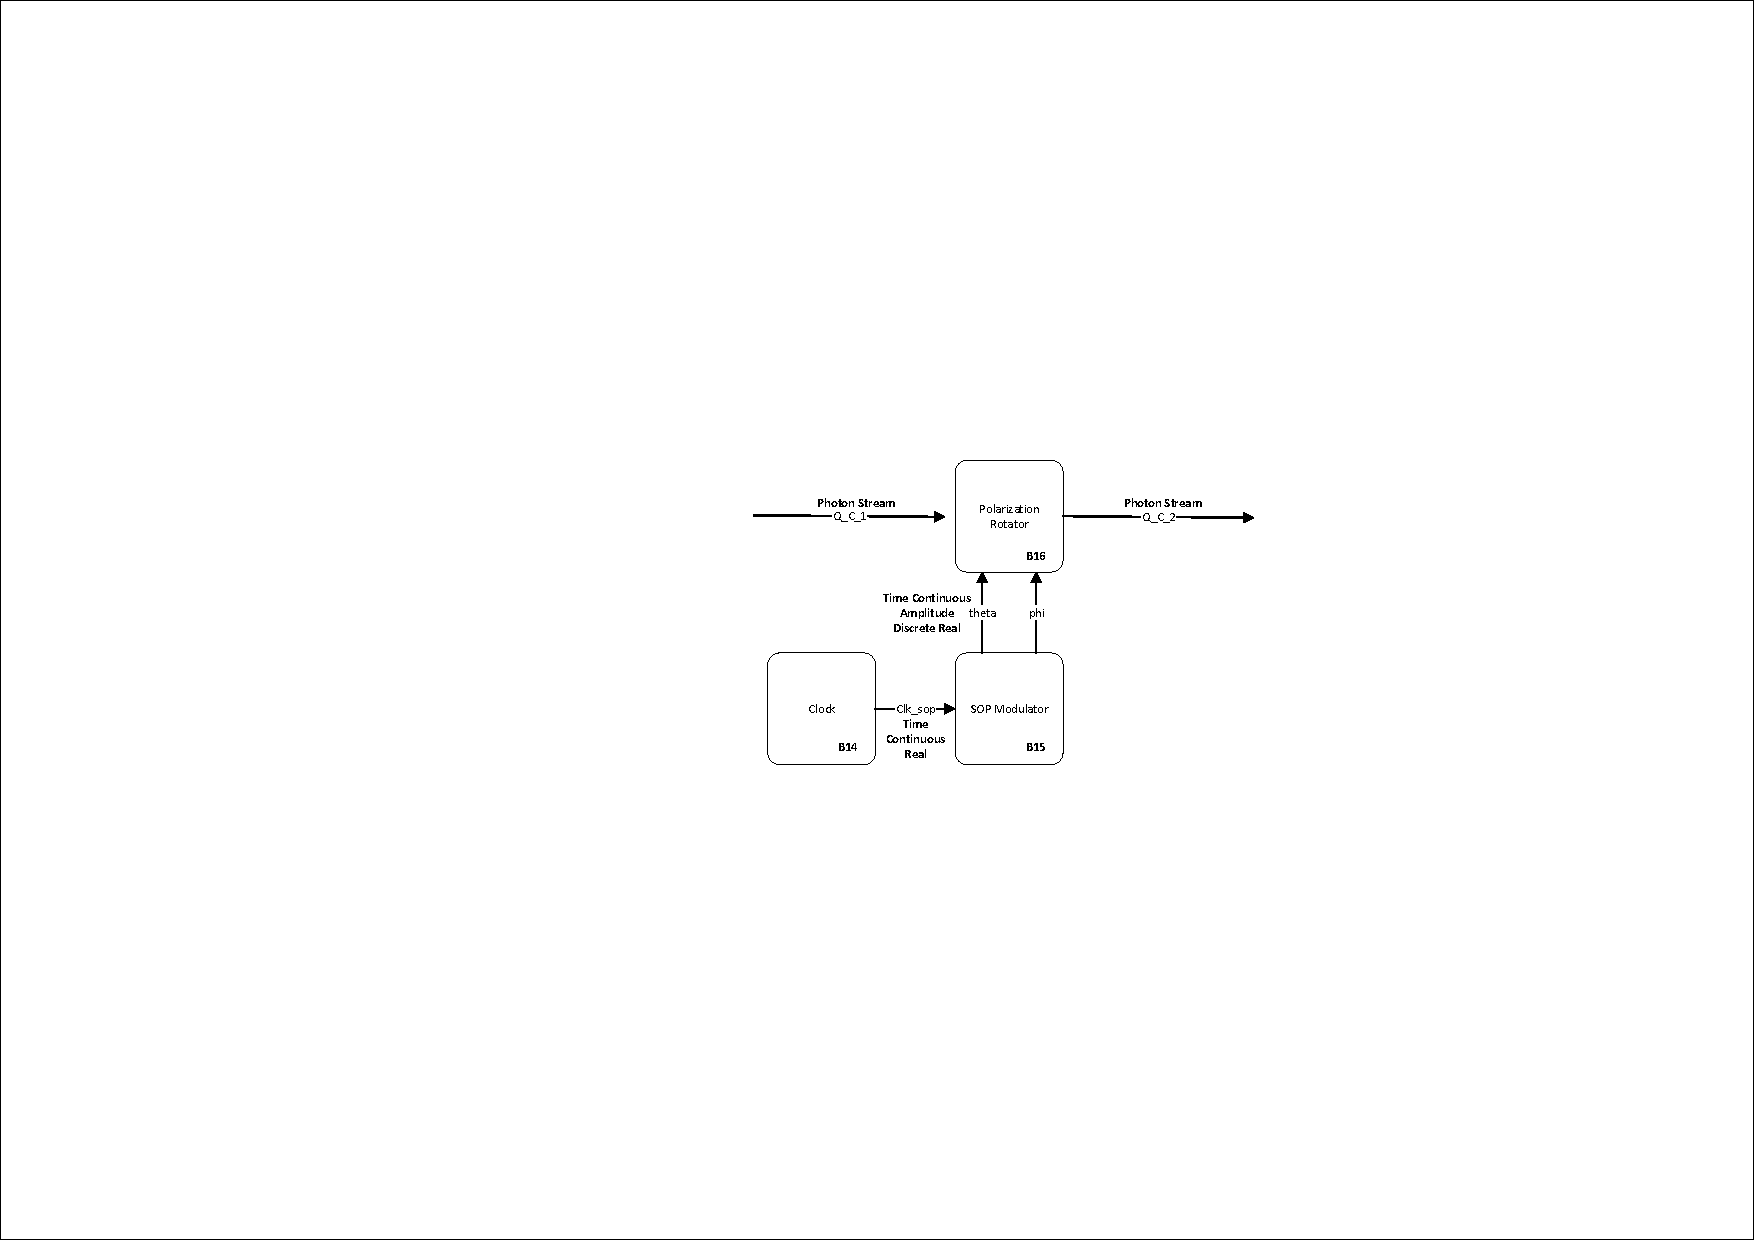
\includegraphics[clip, trim=9cm 7.0cm 5cm 7.5cm, width=0.80\textwidth]{./sdf/bb84_with_discrete_variables/figures/Simulation_sop.pdf}
    \caption{Quantum channel diagram. }\label{sop_channel}
\end{figure}

Now, it is important to calculate the QBER as a function of the rotation angle $\theta$. In order to do that, it was simulated a deterministic SOP modulation, in which the $\theta$ angle varies over the time. In figure \ref{qber} is presented the variation in the value of QBER with respect with theta changes from $0^\circ$ to $45^\circ$. Theoretically, QBER corresponds to the probability of errors in the channel. Which means that in practice this probability corresponds to the probability of a photon following the wrong path in the polarization beam splitter immediately before the detection circuit.

\begin{figure}[h]
    \centering
        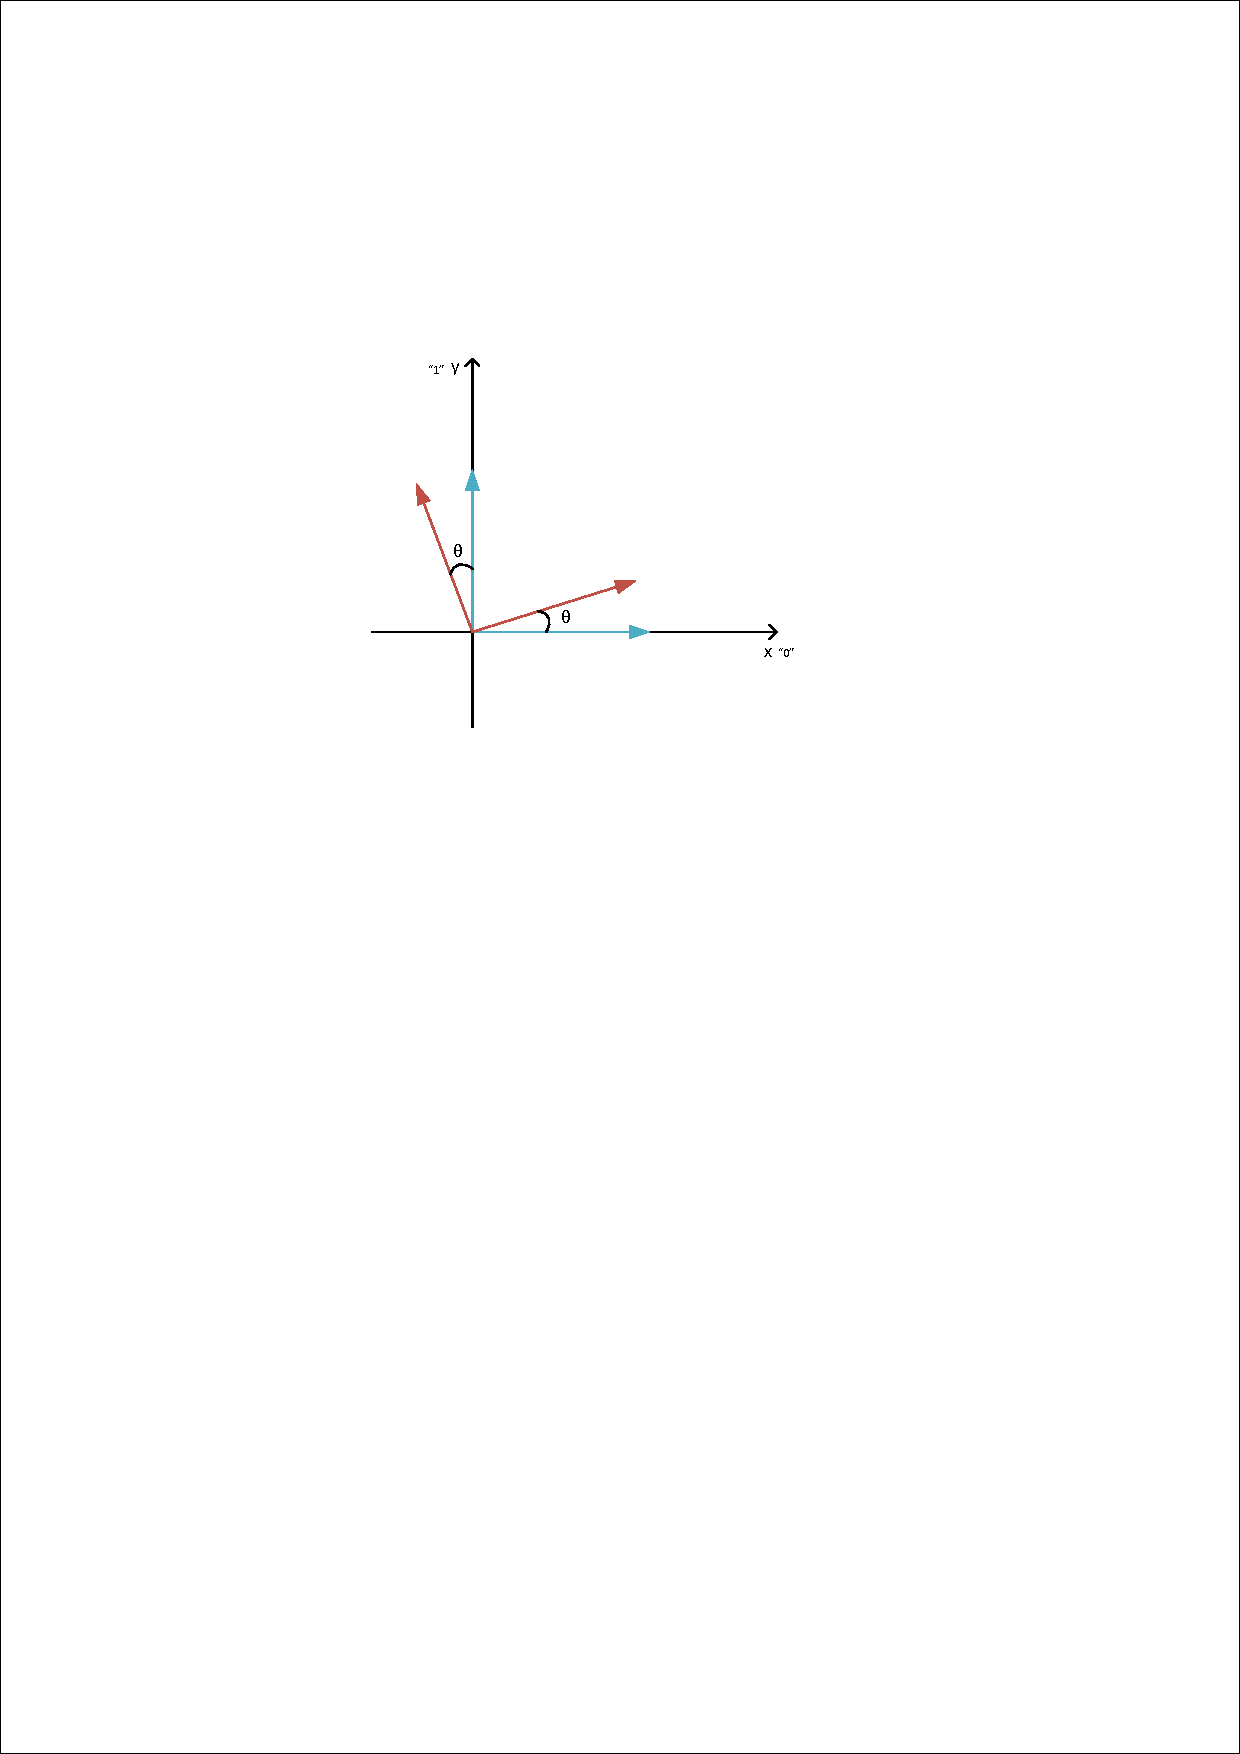
\includegraphics[clip, trim=4cm 17.0cm 5cm 5cm, width=0.80\textwidth]{./sdf/bb84_with_discrete_variables/figures/prob_qber.pdf}
    \caption{Representation of two orthogonal states rotated by an angle $\theta$.}\label{rep_rotation}
\end{figure}

Figure \ref{rep_rotation} presents the graphical representation of two orthogonal states rotated by an angle $\theta$. This rotation is induced by the SOP modulator block which selects a deterministic $\theta$ and $\phi$ angles that do not change over the time. This same rotation is applied for all sequential samples. From figure \ref{rep_rotation} the theoretical QBER can be calculated using the following equation:

\begin{equation}\label{eq:qber}
  QBER = P(0)P(1|0)+P(1)P(0|1).
\end{equation}

Since we have been using a polarization beam splitter 50:50,

\begin{equation*}
  P(0) = P(1) = \frac{1}{2}.
\end{equation*}

This way,
\begin{eqnarray}\label{eq:qber_final}
% \nonumber % Remove numbering (before each equation)
   QBER & = & \frac{1}{2}sin^2(\theta)+ \frac{1}{2}sin^2(\theta)\\
   QBER & = & sin^2(\theta).
\end{eqnarray}

 In figure \ref{qber} are represented two curves: QBER calculated from simulated data and QBER calculated using theoretical model from equation \ref{eq:qber_final}. Furthermore, the cross correlation coefficient between the two signals was calculated using a function from MATLAB \textit{xcorr(x,y,'coeff')} which the result is $99.92\%$. From that, we can conclude that the QBER calculated from simulated data follows the theoretical curve with high correlation. Nevertheless, the error bars presented in figure \ref{qber} were calculated based on a confidence interval of $95\%$.

\begin{figure}[h]
    \centering
        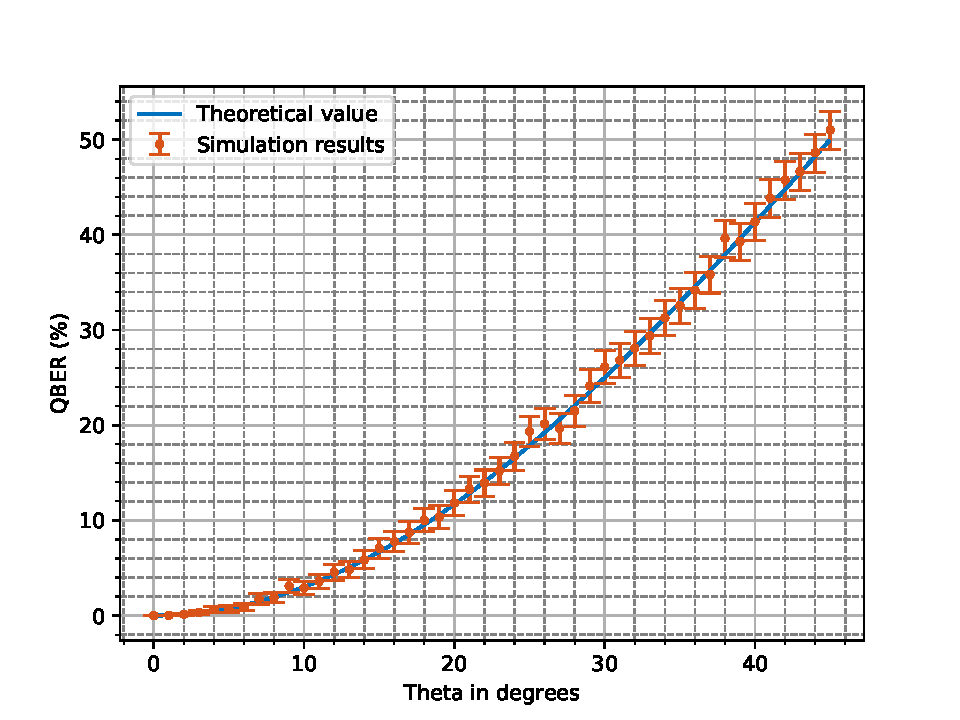
\includegraphics[clip, trim=0.5cm 0.0cm 0.5cm 1cm, width=0.80\textwidth]{./sdf/bb84_with_discrete_variables/figures/QBER_vs_theta_normal_scale.pdf}
    \caption{QBER evolution in relation with deterministic SOP drift.}\label{qber}
\end{figure}

\begin{figure}[H]
    \centering
        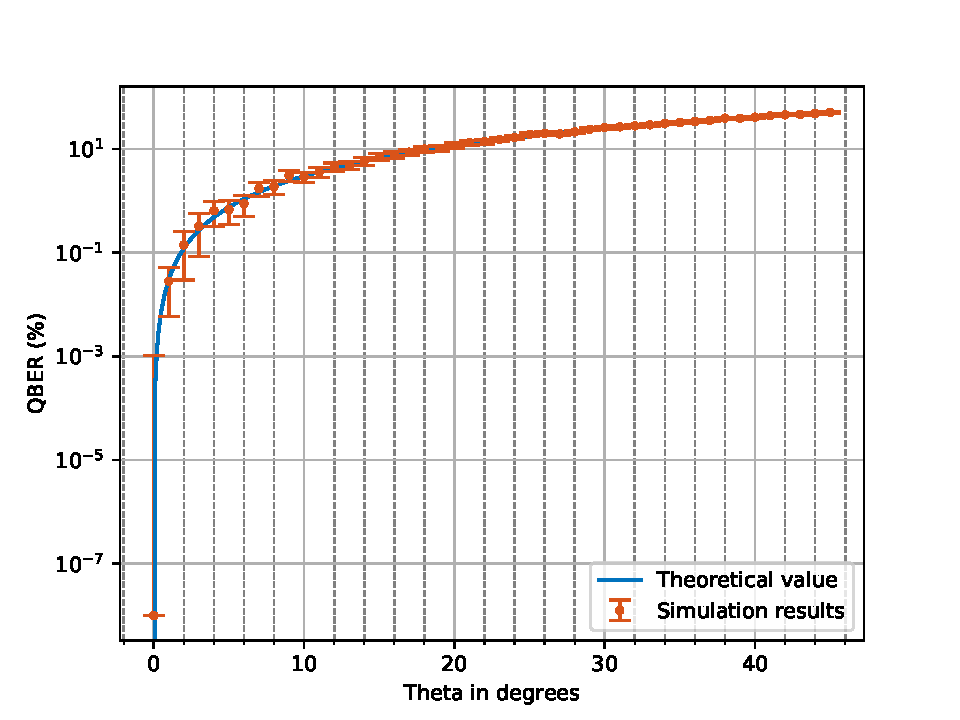
\includegraphics[clip, trim=0.2cm 0.0cm 0.5cm 1cm, width=0.80\textwidth]{./sdf/bb84_with_discrete_variables/figures/qber_vs_theta_all.pdf}
    \caption{QBER evolution in relation with deterministic SOP drift in log scale.}\label{qber_log}
\end{figure}

\begin{figure}[H]
    \centering
        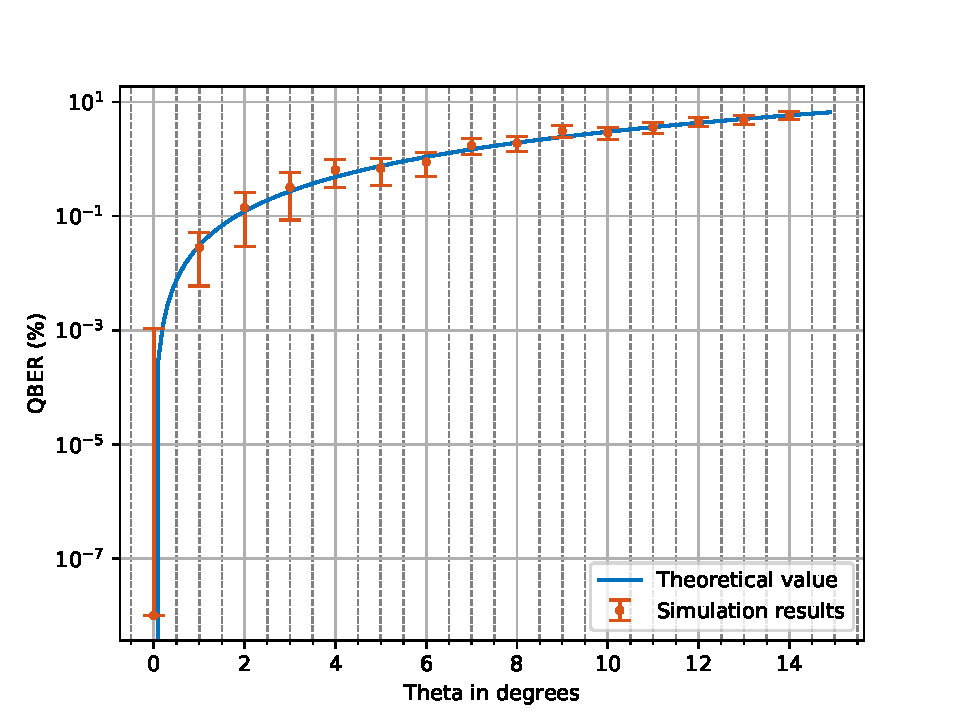
\includegraphics[clip, trim=0.2cm 0.0cm 0.5cm 1cm, width=0.80\textwidth]{./sdf/bb84_with_discrete_variables/figures/QBER_vs_theta_upto15.pdf}
    \caption{QBER evolution in relation with deterministic SOP drift scaled.}\label{qber_log_scaled}
\end{figure}
\newpage

\subsection{Open Issues}
\begin{enumerate}
    \item Estimation of the photons received rate (raw key rate), from the \textrm{SSPR} signal.
    \item Estimation of the key rate after basis reconciliation, from \textrm{MI\_B}.
    \item Include the random polarization rotations in the communication channel.
    \item Implementation of the control system for polarization rotations.
    \item Implementation of a \textrm{QBER} estimation protocol.
    \item Insertion of a new block in \textrm{Bob\_qkd} super block, after the DEMUX\_2\_1 so that we can choose the bits that are going to be used in \textrm{BER} estimation.
    \item Implementation of the scrambling algorithm in order to spread the errors.
    \item Implementation of the cascade for error correction.
    \item Implementation of the output which represents the final key that is built.
    \item Introduce EVE in simulation as shown in figure \ref{toplevelsimulation2}.
        \begin{figure}[H]
        	\centering
        	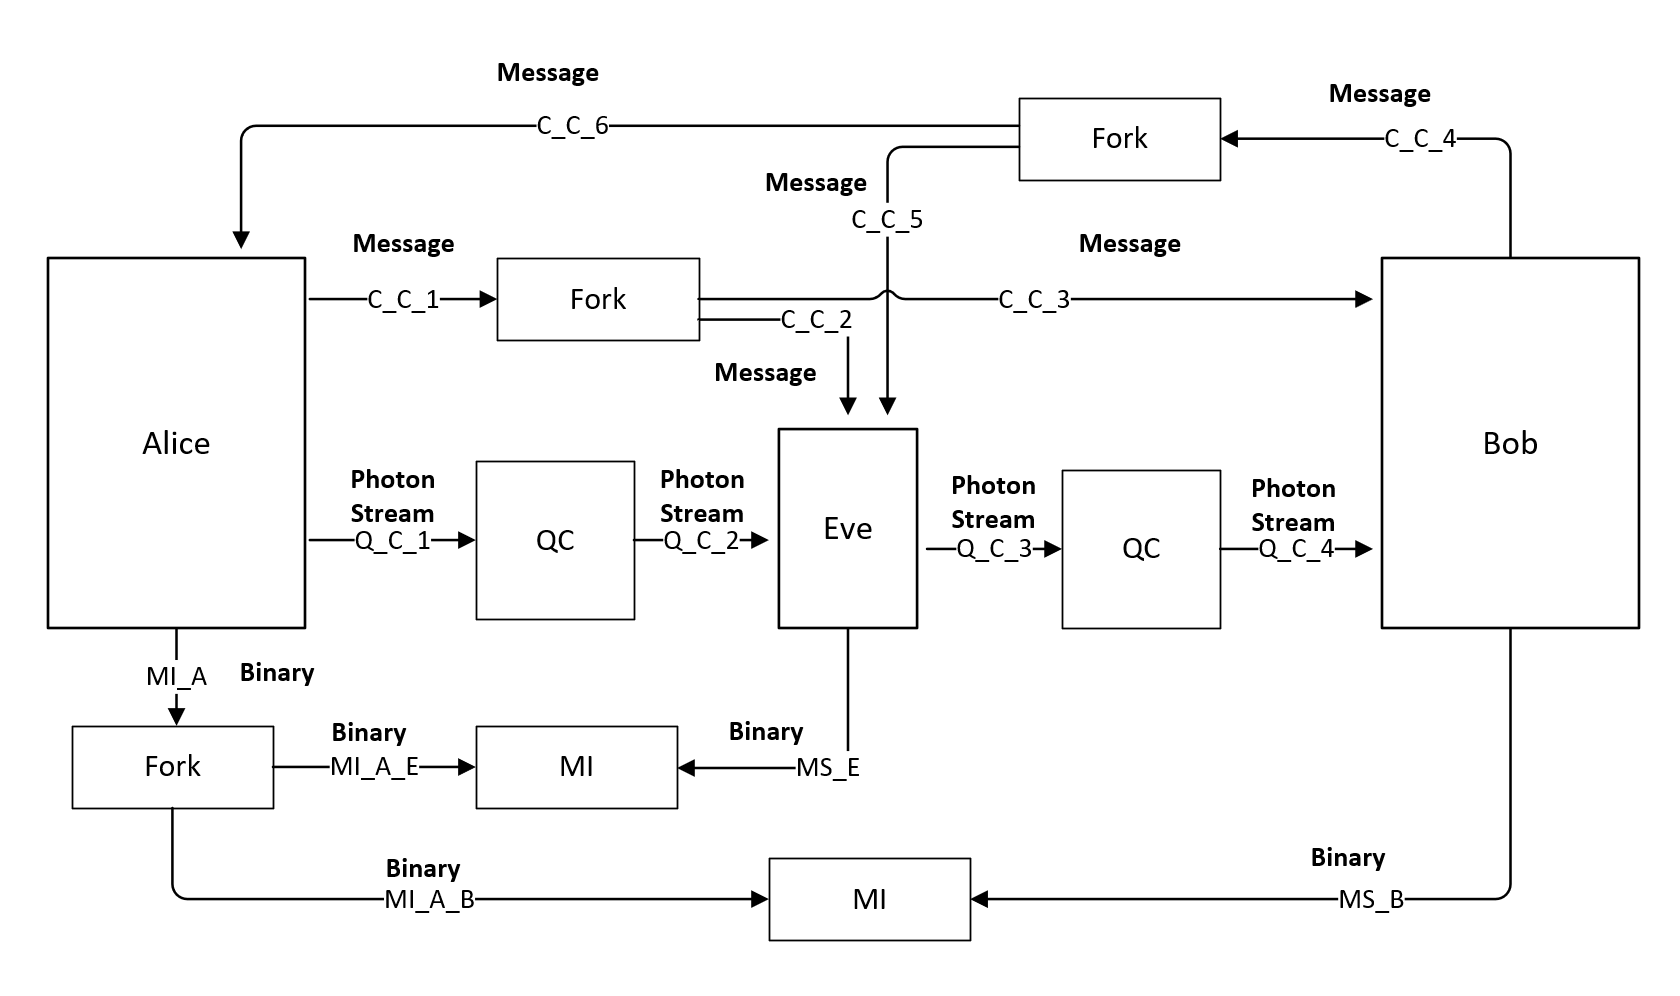
\includegraphics[width=1.0\textwidth, height=9cm]{./sdf/bb84_with_discrete_variables/figures/toplevel_simulation.png}
        	\caption{Simulation diagram at a top level}\label{toplevelsimulation2}
        \end{figure}
    \item Analyze different strategies for Eve.
    \item Experimental Implementation.
\end{enumerate}



\newpage


% COLOCAR ESTAS REFERÊNCIAS NUM FICHEIRO BIB
%
%\begin{thebibliography}{2}
%	\bibitem{BB84}
%	Bennett, C. H. and Brassard,
%	G. Quantum Cryptography: Public key distribution and coin tossing.
%	International Conference on Computers, Systems and Signal Processing, Bangalore, India, 10-12 December 1984, pp. 175-179.
%	
%	\bibitem{SURV}
%	Mart Haitjema, A Survey of the Prominent Quantum Key Distribution Protocols
%	
%	\bibitem{iqo}
%	Christopher Gerry, Peter Knight, "Introductory Quantum Optics" Cambridge University Press, 2005
%	
%	\bibitem{SPREADING}
%	Varadarajan, S., Ngo, H. Q., \& Srivastava, J. (n.d.). An Adaptive , Perception-Driven Error Spreading Scheme in Continuous Media Streaming.
%	
%\end{thebibliography}

% bibliographic references for the section ----------------------------
\clearpage
\printbibliography[heading=subbibliography]
\end{refsection}
\addcontentsline{toc}{subsection}{Bibliography}
\cleardoublepage
% --------------------------------------------------------------------- 